\begin{surferPage}[Sextic (30 Cusps)]{The Barth Sextic with 30 Cusps}
    Dup\u{a} ce Wolf Barth a construit sextica cu num\u{a}rul maxim posibil de
    singularit\u{a}\c{t}i, $65$ (vezi o alt\u{a} suprafa\c{t}\u{a} din aceast\u{a} galerie),
    \c{s}i doi dintre doctoranzii lui au construit noi recorduri mondiale
    \^{i}n grade superioare, el a inceput s\u{a} considere problema num\u{a}rului 
    maxim de puncte cuspidale pe o suprafa\c{t}\u{a} de grad dat.
 
  Construc\c{t}ia lui Barth a unei sextice cu $65$ de singularit\u{a}\c{t}i de tip  $A_1^{+-}$ 
  (conuri duble) poate fi adaptat\u{a} la puncte cuspidale, ob\c{t}in\^{a}nd \^{i}n acest fel 
  $30$ de astfel de puncte: 
    \[P_6 - \alpha \cdot K^3=0,\]
  unde $P_6$ sunt planurile de simetrie ale icosahedrului, ca in cealalt\u{a} 
  sextic\u{a} a lui Barth. La fel ca acolo, $K$ este ecua\c{t}ia sferei unitate:
    \vspace*{-0.4em}
    \begin{center}
      \begin{tabular}{c@{\ }c@{\ }c@{\ }c}
        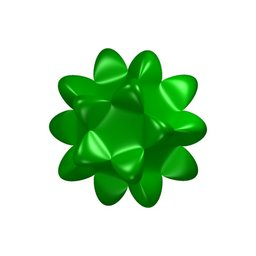
\includegraphics[height=1.2cm]{./../../common/images/barthsextic_30A2}
        &
        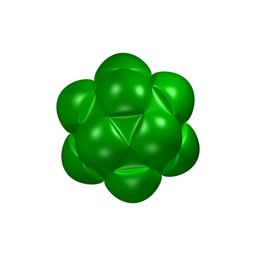
\includegraphics[height=1.2cm]{./../../common/images/barthsextic_30A2_3}
        &
        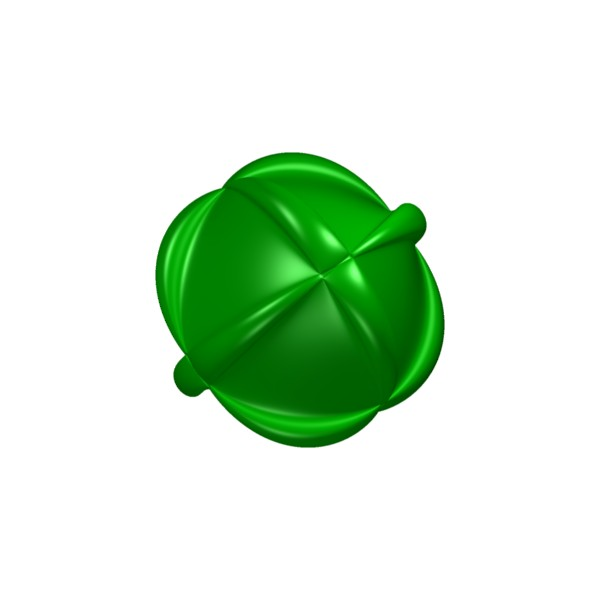
\includegraphics[height=1.2cm]{./../../common/images/barthsextic_30A2_5}
        &
        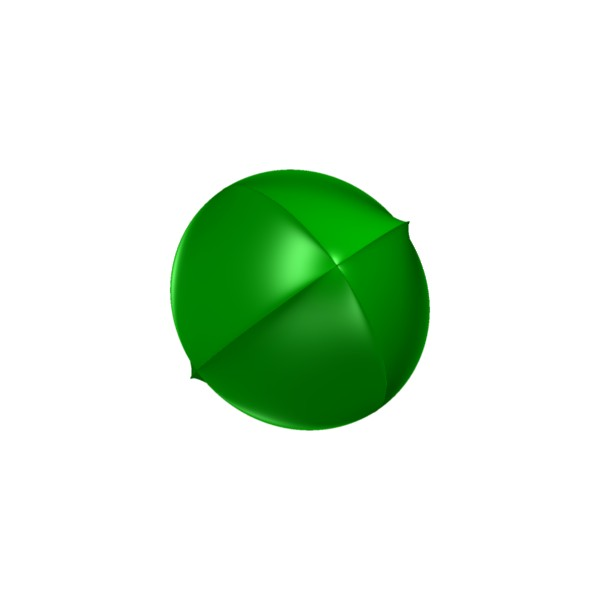
\includegraphics[height=1.2cm]{./../../common/images/barthsextic_30A2_6}
      \end{tabular}
    \end{center}    
    \vspace*{-0.3em}
    Acesta este recordul mondial actual pentru num\u{a}rul maxim de puncte cuspidale reale
    pe o sextic\u{a}. Pentru puncte cuspidale complexe, recordul este de $36$.
  
    
\end{surferPage}
